\id{МРНТИ 61.01.94}

\begin{articleheader}
\sectionwithauthors{М.А. Джетимов, Л.К. Ыбраймжанова, Н.А. Бектенов, Э.А. Камбарова, С.А. Маманова}{ОЧИСТКА СТОЧНЫХ ВОД МОДИФИЦИРОВАННЫМИ ПРИРОДНЫМИ СОРБЕНТАМИ}

{\bfseries \textsuperscript{1}М.А. Джетимов\textsuperscript{\envelope },
\textsuperscript{2}Л.К. Ыбраймжанова, \textsuperscript{3}Н.А. Бектенов,}

{\bfseries \textsuperscript{4}Э.А. Камбарова, \textsuperscript{5}С.А.
Маманова}
\end{articleheader}

\begin{affiliation}
\textsuperscript{1,2,5}Жетысуский университет имени И.Жансугурова,
г.Талдыкорган, Казахстан,

\textsuperscript{3}Казахский национальный педагогический университет
имени Абая, г. Алматы, Казахстан,

\textsuperscript{4}Таразский региональный университет им М.Х.Дулати, г.
Тараз, Казахстан

\raggedright {\bfseries \textsuperscript{\envelope }}Корреспондент-автор: \href{mailto:make._d_61@mail.ru}{\nolinkurl{make.\_d\_61@mail.ru}}
\end{affiliation}

В данной статье представлены результаты исследования применения
комплексных природных минеральных сорбентов на основе
бентонит-монтмориланита, диатомита и цеолита распространенных у подножья
Жетысуского Алатау для очистки и кондиционирования питьевой воды и
очистки сточных вод от тяжелых металлов и других примесей.

Изучен физико-химический, минералогический состав природных сорбентов и
адсорбционная эффективность полученных комбинированных сорбентов,
обнаружено увеличение сорбционной активности в зависимости от состава
сорбента и влияния модификации сорбентов от температуры обжига. Для
повышения адсорбционной способности сорбентов при термообработке
использовали механизм термической активации, что обусловлено удалением
адсорбированной и конституционной воды, то есть увеличение общей
пористости. Близко к термической активации стоит метод гидротермального
модифицирования природных сорбентов - обработка в парах воды при высоких
температурах и давлении.

Научной и практической ценностью нашего исследования, является получение
модификации сорбента, для очистки воды бытовых и промстоков, с
единовременной адсорбцией, содержащихся в сточной воде химических и
микробиологических загрязнений, способствующего обеззараживанию и
умягчению воды, повышающее степень насыщения обработанной воды солями
кальция, магния и микроэлементами не требующего для использования
сложного оборудования. Результатом исследования является создание
модифицированного комплекса из природных сорбентов с очищающей
способностью по значению ПДК.

Проводимых экспериментах по использованию природных минеральных
сорбентов, в процессах очистки воды от загрязнений выявлены существенные
различия в эффективности рассмотренных сорбентов, определяемые их
минеральным составом, микроструктурой, сорбционной емкостью и наличием
каталитической активности.

{\bfseries Ключевые слова:} цеолит, бентонит, диатомит, сорбенты,
адсорбция, тяжелые металлы.

\begin{articleheader}
{\bfseries МОДИФИКАЦИЯЛАНҒАН ТАБИҒИ СОРБЕНТТЕРМЕН АҒЫНДЫ СУЛАРДЫ ТАЗАЛАУ}

{\bfseries \textsuperscript{1}М.А. Джетимов\textsuperscript{\envelope },
\textsuperscript{2}Л.К. Ыбраймжанова, \textsuperscript{3}Н.А. Бектенов,}

{\bfseries \textsuperscript{4}Э.А. Камбарова, \textsuperscript{5}С.А.
Маманова}
\end{articleheader}

\begin{affiliation}
\textsuperscript{1,2,5} І.Жансүгіров атындағы Жетісу университеті,
Талдықорған қ., Казақстан,

\textsuperscript{2}Казахский национальный педагогический университет
имени Абая, Алматы, Қазақстан,

\textsuperscript{4}М.Х. Дулати атындағы Тараз өңірлік университеті,
Тараз қ., Қазақстан,

e-mail:
\href{mailto:make._d_61@mail.ru}{\nolinkurl{make.\_d\_61@mail.ru}}
\end{affiliation}

Бұл мақалада Жетісу (Жоңғар) Алатауының аласа тауларында цеолит,
бентонит саздары және диатомит негізіндегі табиғи минералды сорбенттерді
ауыз суды тазарту және кондиционерлеу және ағынды суларды сульфаттардан,
бикарбонаттардан, нитраттардан, ауыр металл иондарынан және басқа да
зиянды қоспалардан тазарту үшін пайдалану тиімділігін зерттеу нәтижелері
келтірілген.

Табиғи сорбенттердің физика-химиялық және минералогиялық құрамы және
алынған аралас сорбенттердің адсорбциялық тиімділігі зерттеліп,
сорбенттің құрамына және сорбенттердің күйдіру температурасына
модификациясының әсеріне байланысты сорбциялық белсенділіктің жоғарылауы
анықталды. Термиялық өңдеу кезінде сорбенттердің адсорбциялық қабілетін
арттыру үшін термиялық белсендіру механизмі қолданылды, ол
адсорбцияланған және конституционалды суды жоюға, яғни жалпы
кеуектіліктің жоғарылауына байланысты. Термиялық активацияға жақын
табиғи сорбенттерді гидротермиялық модификациялау әдісі -- жоғары
температура мен қысымда су буында өңдеу.

Зерттеу жұмысымыздың ғылыми-практикалық құндылығы судың құрамындағы
химиялық және микробиологиялық ластаушы заттарды бір мезгілде сорбциялай
отырып, суды зарарсыздандыруға және жұмсартуға, тазартылған судың
кальциймен қанығу дәрежесін арттыруға көмектесетін ағынды суларды
тазартуға арналған сорбенттің модификациясын алу болып табылады, магний
тұздары мен микроэлементтер, күрделі жабдықты пайдалануды қажет
етпейтін. Техникалық нәтиже химиялық және микробиологиялық ластаушы
заттарды сорбциялау қабілеті бар табиғи адсорбенттердің
модификацияланған кешенін жасаудан, суды зарарсыздандырудан және
жұмсартудан, оны кальций, магний, натрий, калий иондарымен, сонымен
қатар микроэлементтермен байытудан тұрады.

Табиғи минералды сорбенттерді суды ластаушы заттардан тазарту
процестерінде қолдану бойынша жүргізілген тәжірибелер минералдық
құрамымен, микроқұрылымымен, сорбциялық қабілетімен және каталитикалық
активтілігімен анықталатын қарастырылып отырған сорбенттердің
тиімділігінде айтарлықтай айырмашылықтарды анықтады.

{\bfseries Түйін сөздер:} цеолит, бентонит, диатомит, сорбенттер,
адсорбция, ауыр металдар.

\begin{articleheader}
{\bfseries WASTEWATER TREATMENT USING MODIFIED NATURAL SORBENTS}

{\bfseries \textsuperscript{1}M.A. Jetimov\textsuperscript{\envelope },
\textsuperscript{2}L.K. Ybraimzhanova, \textsuperscript{3}N.A.
Bektenov,}

{\bfseries \textsuperscript{4}E.A.~Kambarova, \textsuperscript{5}S.A.
Mamanova}
\end{articleheader}

\begin{affiliation}
\textsuperscript{1,2,5}Zhetysu University named after I. Zhansugurov,
Taldykorgan, Kazakhstan,

\textsuperscript{3}Abai Kazakh National Pedagogical University, Almaty,
Kazakhstan,

\textsuperscript{4}M.Kh.Dulati Taraz Regional University, Taraz,
Kazakhstan,

e-mail: \href{mailto:make._d_61@mail.ru}{\nolinkurl{make.\_d\_61@mail.ru}}
\end{affiliation}

This article presents the results of a study of the effectiveness of
using natural mineral sorbents based on zeolite, bentonite clays and
diatomite in the low mountains of Zhetysu (Dzungar) Alatau for
purification and conditioning of drinking water and wastewater treatment
from sulfates, bicarbonates, nitrates, heavy metal ions and other
harmful impurities .

The physicochemical and mineralogical composition of natural sorbents
and the adsorption efficiency of the resulting combined sorbents were
studied, and an increase in sorption activity was found depending on the
composition of the sorbent and the influence of modification of the
sorbents on the firing temperature. To increase the adsorption capacity
of sorbents during heat treatment, the mechanism of thermal activation
was used, which is due to the removal of adsorbed and constitutional
water, that is, an increase in total porosity. Close to thermal
activation is the method of hydrothermal modification of natural
sorbents - treatment in water vapor at high temperatures and pressure.

The scientific and practical value of our research is to obtain a
modification of the sorbent for wastewater purification, with
simultaneous sorption of chemical and microbiological contaminants
contained in water, promoting disinfection and softening of water,
increasing the degree of saturation of the treated water with calcium,
magnesium salts and microelements, not requiring for use complex
equipment. The technical result consists in creating a modified complex
of natural adsorbents with the sorbing ability of chemical and
microbiological contaminants, disinfecting and softening water,
enriching it with calcium, magnesium, sodium, potassium ions, as well as
microelements.

Experiments conducted on the use of natural mineral sorbents in water
purification processes from contaminants have revealed significant
differences in the effectiveness of the considered sorbents, deter-mined
by their mineral composition, microstructure, sorption capacity and the
presence of catalytic activity.

{\bfseries Keywords:} zeolite, bentonite, diatomite, sorbents, adsorption,
heavy metals.

\begin{multicols}{2}
{\bfseries Введение.} В настоящее время проблема очистки сточных вод
актуальна для всех стран мира, включая Республику Казахстан. Одним из
основных загрязнителей природных вод являются ионы тяжелых металлов,
поступающие в сточные воды из черной и цветной металлургии,
горнодобывающей и химической промышленности {[}1-4{]}.

Известны многочисленные способы очистки питьевой и сточной воды, но
среди них методы адсорбции с использованием природных адсорбентов просты
и эффективны. Преимуществами этих методов является высокая эффективность
очистки сточных вод, содержащие различные химические вещества. В
литературе появляются все больше сообщений об эффективности
использования природных сорбентов для удаления дисперсных примесей,
ионов тяжелых металлов, нефти и нефтепродуктов, радиоактивных
загрязнений подземных и надземных вод {[}1, 2{]}.

В качестве сорбентов используются активированные угли, зола, шлаки,
колбы, опилки, минеральные сорбенты - глины и другие. Первоначальные
исследования показали, что основным недостатком природных глинистых
минералов является их низкая сорбционная способность. Кроме того,
вышеупомянутые сорбенты являются либо одноразовыми, либо трудными для
удаления, некоторые из них являются токсичными {[}3,4,5{]}.

Многие природные минералы обладают сорбционными свойствами. Цеолиты и
породы, сложенные преимущественно опалом (фляга, диатомит, трепел),
широко используются в качестве природных материалов, перспективных для
извлечения ионов цветных и тяжелых металлов из водных растворов {[}6,
7{]}.

Многолетние исследования ученых Загребского университета Кармен Маргета,
Наташа Забуковец Логар, Марио Шилег и Анамария Фаркаш, использование
природных цеолитов для очистки сточных вод является наиболее
перспективным {[}8{]}.

Значение тяжелых металлов (Fe Zn, Pb, Cr, Cd, Cu, и др.) в загрязненных
водах бытовых и промстоков и их очистка является серьезной экологической
проблемой {[}8, 9{]}.

Природные сорбенты широко исследовались вместе с другими методами, в том
числе химическими: ионообменная, коагуляционная флокуляция, мембранная
фильтрация, площадная, адсорбционная, флотация и электрохимические
методы {[}8{]}. Наши исследования природных цеолитов в качестве
адсорбентов при очистке сточных вод, подтвердили их свойства и значение
модификации.

Представляется весьма перспективным использование природных сорбентов,
месторождения которых находятся на территории Республики Казахстан. У
модифицированного сорбента эффективность адсорбционной емкости достигает
70-80\%, что зависит от химического состава природного адсорбента,
размера адсорбционной емкости и ее доступности, а также от химической
формы его присутствия в среде.

Поэтому перспективным природным сорбентом для очистки питьевых и сточных
вод промышленных предприятий и предприятий коммунального хозяйства
является цеолит месторождения Майтобе в нижней части западного отрога
Жетысу Алатау и бентонитовые глины месторождения Мукры области Жетісу
Республики Казахстан.

Интересным направлением повышения эффективности и универсальности
сорбентов на основе природных материалов является получение
комбинированных сорбентов из цеолита и бентонита.

Целью исследования является получение модифицированных адсорбентов на
основе цеолита, диатомита и бентонита, исследование их физико-химических
параметров и сорбционных свойств, определения эффективности при очистке
бытовых и промышленных сточных вод, способствующих обеззараживанию и
умягчению воды, при этом не требующих использования дорогостоящей и
сложной технологии.

{\bfseries Материалы и методы.} В ходе исследования методом количественного
химического и рентгенофазного анализа, изучен химический состав цеолита
Майтобинского месторождения и бентонитовой глины Мукрынского
месторождения, расположенной в области Жетісу Республики Казахстан.
\end{multicols}

\begin{figure}[H]
	\centering
	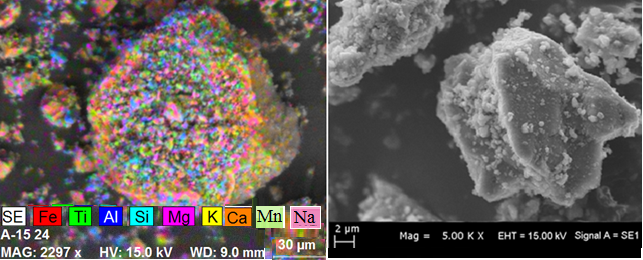
\includegraphics[width=0.95\textwidth]{media/chem/image1}
	\caption*{Рис. 1 - Результаты рентгенофазного анализа сканирующим
электроным микроскопом «EVO 50 XVP» (Carl Zeiss) с зондовой системой
микроанализа «INCA Energy - 350» (Oxford Instruments), цеолита
месторождения Майтобе}
\end{figure}

\begin{multicols}{2}
По данным рентгенофазного и количественно-химического анализа цеолиты
относятся к
водным~\href{https://ru.wikipedia.org/wiki/\%D0\%90\%D0\%BB\%D1\%8E\%D0\%BC\%D0\%BE\%D1\%81\%D0\%B8\%D0\%BB\%D0\%B8\%D0\%BA\%D0\%B0\%D1\%82\%D1\%8B}{алюмосиликатам}~\href{https://ru.wikipedia.org/wiki/\%D0\%9A\%D0\%B0\%D0\%BB\%D1\%8C\%D1\%86\%D0\%B8\%D0\%B9}{кальция}~и~\href{https://ru.wikipedia.org/wiki/\%D0\%9D\%D0\%B0\%D1\%82\%D1\%80\%D0\%B8\%D0\%B9}{натрия}~из
подкласса
каркасных~\href{https://ru.wikipedia.org/wiki/\%D0\%A1\%D0\%B8\%D0\%BB\%D0\%B8\%D0\%BA\%D0\%B0\%D1\%82\%D1\%8B_(\%D0\%BC\%D0\%B8\%D0\%BD\%D0\%B5\%D1\%80\%D0\%B0\%D0\%BB\%D1\%8B)}{силикатов},
со стеклянным или
перламутровым~\href{https://ru.wikipedia.org/wiki/\%D0\%91\%D0\%BB\%D0\%B5\%D1\%81\%D0\%BA}{блеском},
известных своей способностью отдавать и вновь
поглощать~\href{https://ru.wikipedia.org/wiki/\%D0\%92\%D0\%BE\%D0\%B4\%D0\%B0}{воду}~в
зависимости от температуры и влажности (Рис. 1).

Исследование с использованием электронного микроскопа с увеличением до 2
мкм показало пустоты, содержащиеся в структуре цеолитной рамки.
Сорбционные емкости заняты крупными ионами и молекулами
H\textsubscript{2}O, что приводит к обмену ионнами и обратимости
дегидратации (Рис. 1).

Кристаллическая решётка цеолита имеет тетраэдрическое строение, а центры
занимают атомы кремния и алюминия, а атомы кислорода находятся на
вершинах тетраэдра. Значение отрицательного заряда атомов кислорода не
пополняется суммарным положительным зарядом атомов алюминия и кремния,
поэтому, тетраэдрическая кристаллическая решетка несет избыточный
отрицательный заряд {[}10{]}.

Внутренние полости цеолитов содержат множество катионов, в основном
щелочных и щелочноземельных металлов, которые могут заменять друг друга.
(Рис. 2).

Химическая формула: Цеолит месторождения Майтобе, имеет общую формулу
(К, Nа) 4CaAl\textsubscript{6}Si\textsubscript{30}O\textsubscript{72} •
24Н\textsubscript{2}О - кристаллический водный алюмосиликат {[}11,
12{]}.

Химический состав цеолита определяли электронным микроскопом «EVO 50
XVP» (Carl Zeiss) с зондовой системой микроанализа «INCA Energy - 350»
(Oxford Instruments): Na\textsubscript{2}O- 1,9-2,3\%;
Fe\textsubscript{2}O\textsubscript{3}- 0,8-1,2\%;
AI\textsubscript{2}O\textsubscript{3}- 12,9-13,2\%; CaO- 1,7-2,3\%;
K\textsubscript{2}O- 4,0-4,9\%; V- 0,001\%; Cu-0,002\%; Rb- 0,001\%;
SiO\textsubscript{2}- 67,2-76,3\%; Мn-0,001\%; Be-0,002\%; As-0,03\%
(Рисунок 1 и 2).

Важной особенностью цеолита месторождения Майтобе, является наличие в их
структуре системы сорбционной емкости и продольных каналов, которые
составляют до 54\% от общего объёма цеолита, что определяет его ценность
как адсорбента {[}13{]}.

Входные отверстия из каналов в полость цеолита, образованные кольцами
атомов кислорода, являются узкими местами каналов. Эти показатели
определяют адсорбционные свойства природного сорбента.
\end{multicols}

\begin{figure}[H]
	\centering
	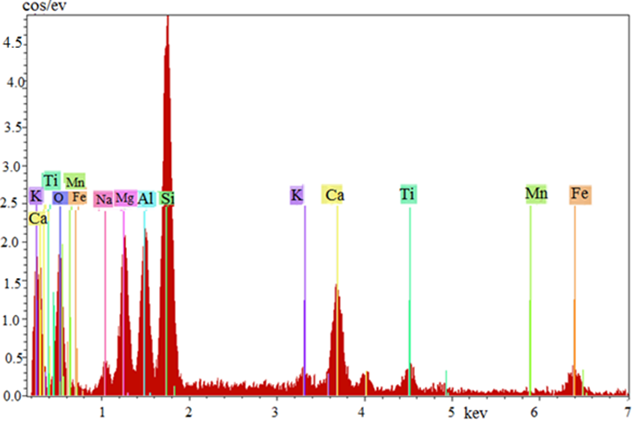
\includegraphics[width=0.8\textwidth]{media/chem/image2}
	\caption*{Рис. 2 - Диаграмма элементного анализа цеолита сканирующим
микроскопом}
\end{figure}

\begin{multicols}{2}
Вторым компонентом природного комбинированного адсорбента является
бентонит-монтмориллонит Мукрынского месторождения. Бентонит представляет
собой глину с 70\% содержанием высокодисперсного слоистого
монтмориллонитового алюмосиликата {[}14{]}.

Бентонитовые глины очищают воду от тяжелых металлов, обесцвечивают,
поглощают неорганические примеси, токсичные хлорорганические соединения
и различные поверхностно-активные вещества.

Химический состав бентонита:
AI\textsubscript{2}O\textsubscript{3}-25,32\%;
SiO\textsubscript{2}-53,42\%; Ca-4,4\%;
Fe\textsubscript{2}O\textsubscript{3}-14,57\%; Mn-0,896\%; Ti-0,28\%;
Cl- 0,75\%; Sr-0,36\% {[}15{]}.

Минерал содержит избыток отрицательного заряда, поэтому он компенсирует
обмен катионов в межслойном пространстве монтмориллонита, что
свидетельствует о высокой гидрофильности исследуемого бентонита. При
опускании бентонита в водный раствор вода проникает через межслойное
пространство монтмориллонита, что вызывает гидратацию последнего,
приводящее к набуханию {[}16{]}.

Бентонит Мукрынского месторождения с катионным обменом
Na\textsuperscript{+}, имеющую щелочную среду и относится к натриевым
бентонитам.

В результате исследования качественного минералогического состава
бентонита было доказано, что монтмориллонит является основным минералом
природного бентонита. На бентонитовой дифрактограмме показано значение
угла вершины 2\textsuperscript{θ} равной 6,06; 19,78; 26,57; 35,18 и
61,98° (Рис. 3).

В рентгеновских дифракционных моделях в монтмориллоните были установлены
отражения в угловом диапазоне 2\textsuperscript{θ}, равном 6,06, а также
2 = 19,78° и 2\textsuperscript{θ} = 26,57° минералла кристаболита,
плагиоклаза, гидромики. Образована структура бентонита из
интерстициальных пространств, где расстояние между слоями равен 12,77 Å.

Результаты и обсуждение. В 2020-2022 года из сорбентов был разработан
модифицированный фильтр из бентонита, цеолита и диатомита взятых в
разных процентых соотношениях (рисунок 4). (0,5 кг) (0,8 кг) (0,5 кг)
\end{multicols}

\begin{figure}[H]
	\centering
	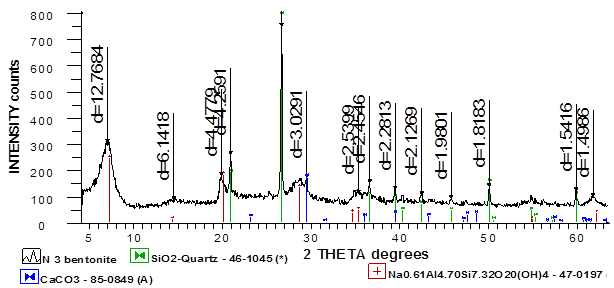
\includegraphics[width=0.9\textwidth]{media/chem/image3}
	\caption*{Рис. 3 - Рентгенограмма образца бентонитовой глины Мукрынского
месторождения области Жетісу}
\end{figure}

\begin{figure}[H]
	\centering
	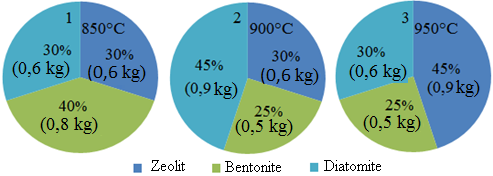
\includegraphics[width=0.7\textwidth]{media/chem/image4}
	\caption*{Рис. 4 - Модифицированные естественные сорбенты на
основе бентонита, цеолита и диатомита, выдержанные при тепературе 850С°,
900С°, 950°С}
\end{figure}

\begin{multicols}{2}
Для проверки эффективности модифицированного естественного сорбента
взяли в разных процентных соотношениях, получили агламерат: 1. Бентонит
40\%, цеолит 30\%, диатомит 30\%; 2. Бентонит 25\%, цеолит 30\%,
диатомит 45\%; 3. Бентонит 25\%, цеолит 45\%, диатомит 30\%.

В дальнейшем из полученной массы изготовили капсулы диаметром 14-16 мм,
длиной 15мм, провели кислотную активацию, использовав
15~\%~H\textsubscript{2}SO\textsubscript{4}, взятых в количестве 50~\%
от воздушно-сухой навески, длительность обработки составила 4 часа. В
муфельной печи при температурах 850 °С С°, 900°С, 950°С градусов провели
термообработку, для увеличения общей пористости. Определение пористости
сорбента проводили по следующей методике. Исследуемые образцы кипятили с
дистиллированной водой на протяжении 1,5--2,0 часов и затем проводили
взвешивание.

Плотность образцов, водопоглощения и пористость рассчитывали по данным
таблицы 1, где: m\textsubscript{0} ~--- масса исследуемых образцов с
подвеской в воде,~г; m\textsubscript{1}~--- масса влажных образцов,~г;
m\textsubscript{2}~---~масса сухих образцов,~г;
m\textsubscript{3}~---~масса подвески,~г.
\end{multicols}

\begin{table}[H]
\caption*{Таблица 1 - Входящие данные для расчета водопоглощения}
\centering
\begin{tabular}{|r|p{0.4\textwidth}|r|r|r|r|}
\hline
\multicolumn{1}{|l|}{№ опыта} & Название материала, tС° & \multicolumn{1}{l|}{m0,г} & \multicolumn{1}{l|}{m1,г} & \multicolumn{1}{l|}{m2,г} & \multicolumn{1}{l|}{m3,г} \\ \hline
1 & Бентонит 40\%, цеолит 30\%, диатомит 30\%; t-850С° & 10,0018 & 31,4312 & 19,0645 & 0,5923 \\ \hline
2 & Бентонит 25\%, цеолит 30\%, диатомит 45\%; t-900С° & 9,6453  & 29,2576 & 16,7312 & 0,4627 \\ \hline
3 & Бентонит 25\%, цеолит 45\%, диатомит 30\%; t-950С° & 9,9459  & 31,2057 & 18,1124 & 0,4134 \\ \hline
\end{tabular}
\end{table}

\begin{multicols}{2}
Определяли оптическую плотность сорбции по метилоранжу на
фотоэлектроколориметре.

В качестве контрольного раствора использовали талую воду. По полученным
оптическим плотностям на основании градуировочного графика определяли
остаточную концентрацию красителя. Сорбционную активность рассчитывали
по формуле~1:

\begin{equation}
X=\frac{(C_1-C_2K)\cdot 0.025}{m}
\end{equation}

где С\textsubscript{1} --- концентрация исходного раствора
красителя,~мг/дм\textsuperscript{3}; С\textsubscript{2} --- концентрация
раствора красителя после взаимодействия с
трепелом,~мг/дм\textsuperscript{3}; К --- коэффициент разбавления; m ---
масса навески комплекса,~г; 0,025 --- объём раствора
метилоранжа,~дм\textsuperscript{3}.
\end{multicols}

\begin{figure}[H]
    \centering
    \begin{subfigure}[t]{0.45\textwidth} % Align at the top
        \centering
        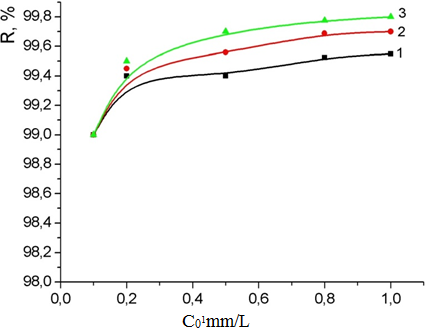
\includegraphics[width=\textwidth]{media/chem/image6}
        \caption*{Рис. 5 - Степень очистки меди от природных сорбентов
спектрофотометром JENWAY 6300. T = 298 K}
    \end{subfigure}
    \hspace{0.05\textwidth} % Adjust horizontal space between the subfigures
    \begin{subfigure}[t]{0.45\textwidth} % Align at the top
        \centering
        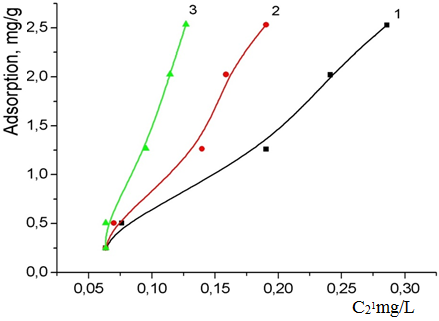
\includegraphics[width=\textwidth]{media/chem/image7}
        \caption*{Рис. 6 - Изотермы сорбции меди комбинированных природных
сорбентов спектрофотометром JENWAY 6300. Т =298К}
    \end{subfigure}
\end{figure}

\begin{multicols}{2}
По результатам эксперимента по адсорбции ионов меди (II) значение
адсорбции было примерно одинаковым на поверхности 3 модифицированных
сорбентов. При максимальной концентрации меди, как видно из рисунка 1,
степень очистки (экстракции) выше 99,6\%. Кроме того, кривые
изотермической адсорбции в 3 композитах ниже, чем адсорбция при низкой
концентрации, при повышенной концентрации кривые резко возрастают,
кривые имеют S-образную форму, что относится к полимолекулярной
адсорбции.
\end{multicols}

\begin{figure}[H]
	\centering
	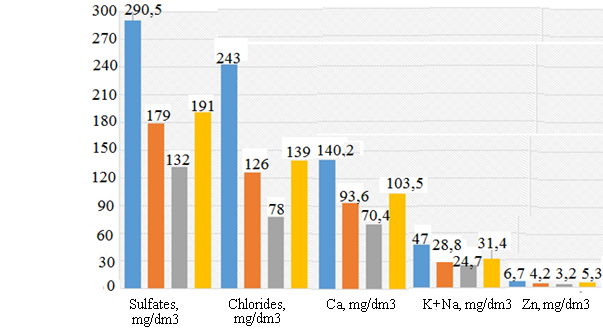
\includegraphics[width=0.8\textwidth]{media/chem/image8}
	\caption*{Рис. 7- Разница хлоридов, сульфатов, Са, К, Na, Zn в неочищенной
и очищенной воде}
\end{figure}

\begin{multicols}{2}
Для проверки эффективности фильтрации воды анализы проводились в
национальной коллективной исследовательской лаборатории по приоритетному
направлению «технологии для углеводородного и горно-металлургического
секторов и смежных сервисных отраслей» акционерного общества «Центр наук
о Земле, металлургии и обогащения» г. Алматы (Рис. 7).

Анализ результатов лабораторного исследования воды показали, что
содержание химических элементов в очищенных водах ниже, чем в
загрязненных водах, их доля в трех пробах различна и соответствует
санитарным нормам (Рис. 7).

По результатам лабораторного анализа проб неочищенных и очищенных воды в
третьей пробе сульфаты, хлориды, бикарбонаты, F, Ca, Sr, K + Na и общая
минерализация значительно ниже, чем фильтра из природных сорбентов
первой и второй пробы (Рис. 7).

Фильтрация воды во второй пробе фильтрата доля стронция снизилась на
62,5\% (0,005 мг/дм\textsuperscript{3}), сульфатов - на 54\% (158
мг/дм\textsuperscript{3}), хлоридов - на 67,9\% (165
мг/дм\textsuperscript{3}), Ca - на 50\% (70 мг/дм\textsuperscript{3}),
общая минерализация - на 59,5\% (338,5 мг/дм\textsuperscript{3}).

Фильтрат воды в первой фильтрационной пробе доля стронция снизилась на
62,5\% (0,035 мг/дм\textsuperscript{3}), сульфатов 158
мг/дм\textsuperscript{3} или 54\%, хлоридов 165 мг/дм\textsuperscript{3}
или 67,9\%, Ca 70 мг/дм\textsuperscript{3} или 50\%.

Анализируя результаты проведенных исследований (диаграмма 5 и 6) мы
пришли к выводу, что по сравнению с первым и третьим образцами фильтра
из природных сорбентов второй более эффективен.

{\bfseries Выводы.} При исследовании сорбционных свойств модифицированных
природных сорбентов трех образцов сделали следующие выводы:

1. Исследования показали предлагаемые нами модефицированные природные
сорбенты наиболее эффективны, чем активированный уголь, зола, шлаки,
фляга, опилки, они нетоксичны, отсутствуют вредные примеси и другие
побочные эффекты.

2. Установлено, что наибольшая эффективность адсорбции ионов тяжелых
металлов наблюдается для сорбента, выдержанного при температуре 900° С.

3. Эффективность очистки водных растворов от ионов тяжелых металлов
(меди) достигает 86,1\%, радионуклидов (стронции) - 66,6\%, от редких
металлов (кадмия) - 44,1\%, от сульфатов 54\%.

4. Положительным показателем сорбентов, является изменение рН, диапазон
от 6,67 до 7,95 повышает эффективность адсорбции сульфатов,
углеводородов, хлоридов, тяжелых, редких металлов и радионуклидов из
сточных вод. Таким образом, предложенный нами сорбент позволит очищать
сточную воду от вредных примесей без снижения параметров очистки.

5. Полученные результаты свидетельствуют о том, что после фильтрации
произошли значительные изменения в составе воды, улучшены его
органолептические характеристики, запах и вкус воды, что соответствуют
санитарным правилам и нормам регулирования.
\end{multicols}

\begin{center}
{\bfseries Литература}
\end{center}

\begin{references}
1.
\href{https://www.sciencedirect.com/science/article/abs/pii/S0304389405002669\#!}{Abidin
Kaya},
\href{https://www.sciencedirect.com/science/article/abs/pii/S0304389405002669\#!}{Ali
Hakan Oren}. Adsorption of zinc from aqueous solutions to bentonite//
\href{https://www.sciencedirect.com/science/journal/03043894}{Journal of
Hazardous Materials}. -2005. -
\href{https://www.sciencedirect.com/science/journal/03043894/125/1}{Vol.
125. - Iss 1--3}. - P. 183-189. DOI 10.1016/j.jhazmat.2005.05.027

2. Алтынбеков Ф.Е. Гигиеническая оценка цеолитов закавказских
месторождений, предлагаемых для совершенствования технологических схем
обработки воды хозяйственно-питьевых водоисточников / Автореф. дисс.
канд.мед. наук. -- Алматы, 1985. -21 с.

3. Kaušpediene D., Kazlauskiene E., Gefeniene A., Binkiene R.,
Comparison of the efficiency of activated carbon and neutral polymeric
adsorbent in removal of chromium complex dye from aqueous solutions //
Journal of Hazardous Materials. -2010. - Vol. 179(1--3). -P. 933--939.
DOI 10.1016/j.jhazmat.2010.03.095

4. Оникиенко С.Б, Земляной А.В., Смуров А.В. и др. Перспективные
направления в применении водоочистительных систем на основе природных
минералов // Мат. Всеармейской научн. конфе­ренции «Военно-медицинские
аспекты экологического обеспече­ния деятельности вооруженных сил
РФ»,-СПб.: ВМедА, 1998.-С. 88-91

5. Bhatnagar A., Sillanpää M. Utilization of agro-industrial and
municipal waste materials as potential adsorbents for water
treatment---a review // Chemical Engineering Journal. -Vol. 157(2-3).
-P. 277--296. DOI 10.1016/j.cej.2010.01.007

6.
\href{https://www.sciencedirect.com/science/article/pii/0956053X9500025U\#!}{Khan}
S.A.,
\href{https://www.sciencedirect.com/science/article/pii/0956053X9500025U\#!}{Riaz-ur-Rehman},
\href{https://www.sciencedirect.com/science/article/pii/0956053X9500025U\#!}{Khan}
M.A. Adsorption of chromium (III), chromium (VI) and silver (I) on
bentonite //
\href{https://www.sciencedirect.com/science/journal/0956053X}{Waste
Management}. -1995.
-\href{https://www.sciencedirect.com/science/journal/0956053X/15/4}{Vol.
1. -Iss. 4}, - P. 271-282. DOI 10.1016/0956-053X(95)00025-U

7. Jetimov M., Yessengabylov I., Maymekov Z., Tokpanov E., S.
Sydykbayeva, Imangazinova Zh., Issayeva G. Sorption characteristics of
zeolite and bentonite natural adsorbents modified complex // NEWS of the
national academy of sciences of the republic of Kazakhstan. Series of
geology and technical sciences. -2020. -- Vol. 4(442). -P. 165-173. DOI
\href{http://dx.doi.org/10.32014/2020.2518-170X.94}{10.32014/2020.2518-170X.94}

8.
\href{https://www.ncbi.nlm.nih.gov/pubmed/?term=Rozi\%C4\%87\%20M\%5BAuthor\%5D&cauthor=true&cauthor_uid=15752783}{Rozić
M}{\bfseries ,}
\href{https://www.ncbi.nlm.nih.gov/pubmed/?term=Cerjan-Stefanovi\%C4\%87\%20S\%5BAuthor\%5D&cauthor=true&cauthor_uid=15752783}{Cerjan-Stefanović
S},~\href{https://www.ncbi.nlm.nih.gov/pubmed/?term=Kurajica\%20S\%5BAuthor\%5D&cauthor=true&cauthor_uid=15752783}{Kurajica
S},~\href{https://www.ncbi.nlm.nih.gov/pubmed/?term=Maeefat\%20MR\%5BAuthor\%5D&cauthor=true&cauthor_uid=15752783}{Maeefat
MR},~\href{https://www.ncbi.nlm.nih.gov/pubmed/?term=Margeta\%20K\%5BAuthor\%5D&cauthor=true&cauthor_uid=15752783}{Margeta
K},~\href{https://www.ncbi.nlm.nih.gov/pubmed/?term=Farkas\%20A\%5BAuthor\%5D&cauthor=true&cauthor_uid=15752783}{Farkas
A}. Decationization and dealumination of clinoptilolite tuff and
ammonium exchange on acid-modified tuff //
\href{https://www.ncbi.nlm.nih.gov/pubmed/15752783}{J Colloid Interface
Sci.} - 2005. - Vol. 284(1).48-56. DOI: 10.1016/j.jcis.2004.09.061

9. Removal of Mn\textsuperscript{2+} ions from drinking water by using
Clinoptilolite and a Clinoptilolite--Fe oxide system / M.K. Doula //
Water Research. - 2006. -Vol. 40(17). - Р. 3167--3176. DOI:
10.1016/j.watres.2006.07.013

10. Kinetic research on the sorption of aqueous lead by synthetic
carbonate hydroxyapatite / H. Xu, L. Yang, P. Wang, Y. Liu, M. Peng //
J. Environ. Manage. - 2008. - V. 86. - Р. 319--328. DOI:
\\10.1016/j.jenvman.2006.12.011

11. Комарова Л.Ф. Физико-химические основы применения природных и
модифицированных сорбентов в процессах очистки воды // Химия и
технология воды, 1998. -Т. 20(1). -С.42-51.

12. Wang S, Peng Y Natural zeolites as effective adsorbents in water and
wastewater treatment // Chem. Engin J. -- 2010. -Vol. 156. -P.11-24.

13. L. Harutyunyan and G. Pirumyan, Purification of waters from anionic
and cationic surfactants by natural zeolite // Chemistry and Biology.
-2015. - Vol. 1. - P. 21--28.

14. Bourliva A., Michailidis K., Sikalidis C., Filippidis A., and
Apostolidis N. Municipal wastewater treatment with bentonite from Milos
Island, Greece //Bulletin of the geological society of Greece. -- 2010.
--Vol. 43(5). --P. 2532-2539. DOI 10.12681/bgsg.11660

15. Jetimov M., Andasbayev E., Sataeva A. Efficiency of using a complex
of modified natural adsorbents for wastewater treatment. In the
collection //The Europe and the Turkic World: Science, Engineering and
Technology Materials of the III International Scientific-Practical
Conference. - 2018. -P. 447-452.

16. Chartterjee T., Chartterjee S., and HanWoo S Enhanced coagulation of
bentonite particles in water by a modified chitosan biopolymer //
Chemical engineering journal. -2009. --Vol. 148. --P. 414-419. DOI
10.1016/j.cej.2008.09.016
\end{references}

\begin{center}
{\bfseries References}
\end{center}

\begin{references}
1.
\href{https://www.sciencedirect.com/science/article/abs/pii/S0304389405002669\#!}{Abidin
Kaya},
\href{https://www.sciencedirect.com/science/article/abs/pii/S0304389405002669\#!}{Ali
Hakan Oren}. Adsorption of zinc from aqueous solutions to bentonite//
\href{https://www.sciencedirect.com/science/journal/03043894}{Journal of
Hazardous Materials}. -2005. -
\href{https://www.sciencedirect.com/science/journal/03043894/125/1}{Vol.
125. - Iss 1--3}. - P. 183-189. DOI 10.1016/j.jhazmat.2005.05.027

2. Altynbekov F.E. Gigienicheskaya otsenka tseolitov zakavkazskikh
mestorozhdenii, predlagaemykh dlya sovershenstvovaniya
tekhnologicheskikh skhem obrabotki vody
khozyaistvenno-pit' evykh vodoistochnikov / Avtoref.
diss. kand.med. nauk. -- Almaty, 1985. -21 s. {[}in Russian{]}

3. Kaušpediene D., Kazlauskiene E., Gefeniene A., Binkiene R.,
Comparison of the efficiency of activated carbon and neutral polymeric
adsorbent in removal of chromium complex dye from aqueous solutions //
Journal of Hazardous Materials. -2010. - Vol. 179(1--3). -P. 933--939.
DOI 10.1016/j.jhazmat.2010.03.095

4. Onikienko S.B, Zemlyanoi A.V., Smurov A.V. i dr. Perspektivnye
napravleniya v primenenii vodoochis-titel' nykh sistem na
osnove prirodnykh mineralov // Mat. Vsearmeiskoi nauchn. konfe¬rentsii
«Voenno-meditsinskie aspekty ekologicheskogo obespeche¬niya
deyatel' nosti vooruzhennykh sil RF»,-SPb.: \\VMedA,
1998.-S. 88-91. {[}in Russian{]}

5. Bhatnagar A., Sillanpää M. Utilization of agro-industrial and
municipal waste materials as potential adsorbents for water
treatment---a review // Chemical Engineering Journal. -Vol. 157(2-3).
-P. 277--296. DOI 10.1016/j.cej.2010.01.007

6.
\href{https://www.sciencedirect.com/science/article/pii/0956053X9500025U\#!}{Khan}
S.A.,
\href{https://www.sciencedirect.com/science/article/pii/0956053X9500025U\#!}{Riaz-ur-Rehman},
\href{https://www.sciencedirect.com/science/article/pii/0956053X9500025U\#!}{Khan}
M.A. Adsorption of chromium (III), chromium (VI) and silver (I) on
bentonite //
\href{https://www.sciencedirect.com/science/journal/0956053X}{Waste
Management}. -1995.
-\href{https://www.sciencedirect.com/science/journal/0956053X/15/4}{Vol.
1. -Iss. 4}, - P. 271-282. DOI 10.1016/0956-053X(95)00025-U

7. Jetimov M., Yessengabylov I., Maymekov Z., Tokpanov E., S.
Sydykbayeva, Imangazinova Zh., Issayeva G. Sorption characteristics of
zeolite and bentonite natural adsorbents modified complex // NEWS of the
national academy of sciences of the republic of Kazakhstan. Series of
geology and technical sciences. -2020. -- Vol. 4(442). -P. 165-173. DOI
\href{http://dx.doi.org/10.32014/2020.2518-170X.94}{10.32014/2020.2518-170X.94}

8.
\href{https://www.ncbi.nlm.nih.gov/pubmed/?term=Rozi\%C4\%87\%20M\%5BAuthor\%5D&cauthor=true&cauthor_uid=15752783}{Rozić
M}{\bfseries ,}
\href{https://www.ncbi.nlm.nih.gov/pubmed/?term=Cerjan-Stefanovi\%C4\%87\%20S\%5BAuthor\%5D&cauthor=true&cauthor_uid=15752783}{Cerjan-Stefanović
S},~\href{https://www.ncbi.nlm.nih.gov/pubmed/?term=Kurajica\%20S\%5BAuthor\%5D&cauthor=true&cauthor_uid=15752783}{Kurajica
S},~\href{https://www.ncbi.nlm.nih.gov/pubmed/?term=Maeefat\%20MR\%5BAuthor\%5D&cauthor=true&cauthor_uid=15752783}{Maeefat
MR},~\href{https://www.ncbi.nlm.nih.gov/pubmed/?term=Margeta\%20K\%5BAuthor\%5D&cauthor=true&cauthor_uid=15752783}{Margeta
K},~\href{https://www.ncbi.nlm.nih.gov/pubmed/?term=Farkas\%20A\%5BAuthor\%5D&cauthor=true&cauthor_uid=15752783}{Farkas
A}. Decationization and dealumination of clinoptilolite tuff and
ammonium exchange on acid-modified tuff //
\href{https://www.ncbi.nlm.nih.gov/pubmed/15752783}{J Colloid Interface
Sci.} - 2005. - Vol. 284(1).48-56. DOI: 10.1016/j.jcis.2004.09.061

9. Removal of Mn\textsuperscript{2+} ions from drinking water by using
Clinoptilolite and a Clinoptilolite--Fe oxide system / M.K. Doula //
Water Research. - 2006. -Vol. 40(17). - Р. 3167--3176. DOI:
10.1016/j.watres.2006.07.013

10. Kinetic research on the sorption of aqueous lead by synthetic
carbonate hydroxyapatite / H. Xu, L. Yang, P. Wang, Y. Liu, M. Peng //
J. Environ. Manage. - 2008. - V. 86. - Р. 319--328. DOI:
\\10.1016/j.jenvman.2006.12.011

11. Komarova L.F. Fiziko-khimicheskie osnovy primeneniya prirodnykh i
modifitsirovannykh sorbentov v protsessakh ochistki vody // Khimiya i
tekhnologiya vody, 1998. -T. 20(1). -S.42-51. {[}in Russian{]}

12. Wang S, Peng Y Natural zeolites as effective adsorbents in water and
wastewater treatment // Chem. Engin J. -- 2010. -Vol. 156. -P.11-24.

13. L. Harutyunyan and G. Pirumyan, Purification of waters from anionic
and cationic surfactants by natural zeolite // Chemistry and Biology.
-2015. - Vol. 1. - P. 21--28.

14. Bourliva A., Michailidis K., Sikalidis C., Filippidis A., and
Apostolidis N. Municipal wastewater treatment with bentonite from Milos
Island, Greece //Bulletin of the geological society of Greece. -- 2010.
--Vol. 43(5). --P. 2532-2539. DOI 10.12681/bgsg.11660

15. Jetimov M., Andasbayev E., Sataeva A. Efficiency of using a complex
of modified natural adsorbents for wastewater treatment. In the
collection //The Europe and the Turkic World: Science, Engineering and
Technology Materials of the III International Scientific-Practical
Conference. - 2018. -P. 447-452.

16. Chartterjee T., Chartterjee S., and HanWoo S Enhanced coagulation of
bentonite particles in water by a modified chitosan biopolymer //
Chemical engineering journal. -2009. --Vol. 148. --P. 414-419. DOI
10.1016/j.cej.2008.09.016
\end{references}

\begin{authorinfo}
\hspace{1em}\emph{{\bfseries Сведения об авторах}}

Джетимов М.А.- кандидат технических наук, преподаватель-лектор,
Жетысуского университета им. И. Жансугурова, Талдыкорган, Казахстан,
e-mail:
\href{mailto:make._d_61@mail.ru}{\nolinkurl{make.\_d\_61@mail.ru}};

Ыбраймжанова Л.К.- магистр технических наук, преподаватель-лектор,
естественнонаучного направления Жетысуского университета им. И.
Жансугурова, Талдыкорган, Казахстан, e-mail:
\href{mailto:ybraymzhanova@mail.ru}{\nolinkurl{ybraymzhanova@mail.ru}};

Бектенов Н.А.- доктор химических наук, профессор, главный научный
сотрудник , АО «Институт химических наук им. А.Б. Бектурова», Алматы,
Казахстан, профессор кафедры химии Казахского национального
педагогического университета имени Абая, Алматы, Казахстан, e-mail:
\href{mailto:bekten_1954@mail.ru}{\nolinkurl{bekten\_1954@mail.ru}};

Камбарова Э.А.- магистр химии, Таразский региональный университет им
М.Х.Дулати, г. Тараз, Казахстан, e-mail:
\href{mailto:ilmira080884@mail.ru}{\nolinkurl{ilmira080884@mail.ru}};

Маманова С.А.- магистр, преподаватель-ассистент, Жетысуского
университета им. И. Жансугурова, Талдыкорган, Казахстан, e-mail:
\href{mailto:Msalta81@mail.ru}{\nolinkurl{Msalta81@mail.ru}}

\hspace{1em}\emph{{\bfseries Information about the authors}}

Jetimov M.A.- Candidate of Technical Sciences, teacher-lecturer, Zhetysu
University named after I. Zhansugurov, Taldykorgan, Kazakhstan, e-mail:
\href{mailto:make._d_61@mail.ru}{\nolinkurl{make.\_d\_61@mail.ru}};

Ybraimzhanova L.K. - Master of Technical Sciences, teacher-lecturer,
Zhetysu University named after I. Zhansugurov, \\ Taldykorgan, Kazakhstan,
e-mail: \href{mailto:ybraymzhanova@mail.ruu}{ybraymzhanova@mail.ru};

Bektenov N.A.- Doctor of Chemical Sciences, Professor, JSC «A.B.
Bekturov Institute of Chemical Sciences»,

Almaty, Kazakhstan, Professor of the Department of Chemistry of the
Kazakh National Pedagogical University named after Abai, Almaty,
Kazakhstan, e-mail:
\href{mailto:bekten_1954@mail.ru}{\nolinkurl{bekten\_1954@mail.ru}};

Kambarova E.A.- Master of Chemistry, M.Kh.Dulati Taraz Regional
University, Taraz, Kazakhstan, e-mail:
\href{mailto:ilmira080884@mail.ru}{\nolinkurl{ilmira080884@mail.ru}}

Mamonova S.A.- Master' s degree, lecturer-assistant of
educational programs of the natural science direction of I. Zhansugurov
Zhetysu University, Taldykorgan, Kazakhstan, e-mail:
\href{mailto:Msalta81@mail.ru}{\nolinkurl{Msalta81@mail.ru}}
\end{authorinfo}
